%!TEX root = main.tex
%----------------------------------------------------------------------------------------
% Configuración
%----------------------------------------------------------------------------------------
\documentclass[11pt, oneside]{book} %Las tesis se imprimen a una cara, por eso está el "oneside"
\usepackage[paperwidth=17cm, paperheight=22.5cm, bottom=2.5cm, right=2.5cm]{geometry} % Configuración de la página
\usepackage{amssymb, amsmath, amsthm} %Paquetes para símbolos matemáticos
\usepackage[spanish, mexico]{babel} %Para que el texto esté en español
\usepackage[utf8]{inputenc} %Para acentos y símbolos
\usepackage{enumerate, enumitem} %Para enumerar páginas
\usepackage{graphicx, pgfplots, pgfplotstable, filecontents, tikz, listings, color, float} %Para gráficos y figuras
\usepackage{csquotes, multirow, libertine, adjustbox, threeparttable} % Para citas y tablas
\usepackage[nottoc]{tocbibind}
% \usepackage[backend=bibtex, style=authoryear, autocite=inline]{biblatex} % Para otro tipo de citación
%\usepackage[backend=biber,style=ieee,citestyle=authoryear]{biblatex} % Para citación utilizando APA
%\DeclareLanguageMapping{spanish}{spanish-ieee}
\pgfplotsset{compat=newest}

% Para hipervínculos
 \usepackage{hyperref}
 \hypersetup{
     colorlinks=false,
     linkcolor=black,
     pdftitle={Tesis},
     pdfauthor={Alan J. Amaya Martínez},
     %bookmarks=true,
     linktocpage=true,
     urlcolor=black,
     allbordercolors = {white}
}

\renewcommand{\lstlistingname}{Algoritmo}

\addto\captionsspanish{
    \renewcommand{\contentsname}
    {Tabla de contenido}
}

\pgfplotsset{compat=newest}

%\addbibresource{FormatoTesis/Referencias/references.bib} %Inserción del archivo de bibliografía
% \nocite{*}

\graphicspath{{Imagenes/}} %Carpeta donde están las imágenes

% Para eliminar guiones y justificar texto
\tolerance=1
\emergencystretch=\maxdimen
\hyphenpenalty=10000
\hbadness=10000
\linespread{1.25} %Para tener interlineado de 1.5 de Word

\begin{document}

%----------------------------------------------------------------------------------------
% Portada
%----------------------------------------------------------------------------------------
\begin{titlepage}
\begin{center}
\textsc{\Large Instituto Tecnológico Autónomo de México}\\[1em]

%Logo ITAM
\begin{figure}[h]
\begin{center}

\includegraphics[scale=0.15]{logo-ITAM.png}
\end{center}
\end{figure}

\textsc{\huge \textbf{Diseño de un Controlador de Velocidad en un Aerogenerador}}\\[2em]

\textsc{\large Tesis}\\[1em]
\textsc{\large que para obtener el título de}\\[1em]
\textsc{\large Ingeniero en Mecatrónica}\\[1em]
\textsc{\large Presenta}\\[1em]
\textsc{\Large Alan Josabet Amaya Martínez}\\[1em]
\textsc{\large Asesor}\\[1em]
\textsc{\large Dr. Rafael Cisneros Montoya}\\[1em]
  
\end{center}
\vspace*{\fill}
\textsc{Ciudad de México \hspace*{\fill} 2024}
\end{titlepage}

\tableofcontents % Tabla de Contenidos
\mainmatter % Empieza la numeración arábiga de las páginas
%----------------------------------------------------------------------------------------
%	Tesis
%----------------------------------------------------------------------------------------
%!TEX root = ../main.tex
\chapter{Introducción} \label{intro_chapter}

En este capítulo se hace un breve recorrido por la situación actual de la energía eólica en el país. 
Además, se introducen los conceptos básicos y principios de funcionamiento de la energía eólica y de 
los aerogeneradores. Se presentan el problema del control de una turbina eólica y la motivación en 
el diseño de un controlador que permita agregar un grado de libertad al sistema de la turbina. 
\\

\noindent En esta tesis se utilizarán indistintamente los términos aerogenerador y turbina eólica 
para referirse al conjunto completo del generador eléctrico, las aspas, el cuerpo de la turbina y 
demás componentes que se detallarán más adelante. 


\section{Contexto}
\noindent En la última década en México se ha observado un incremento en el consumo de energía primaria 
proveniente de fuentes renovables. Del 2012 al 2022 se registró un incremento del 5.24\% a 8.96\% 
la proporción del consumo de energía primaria cuyo origen se puede considerar renovable (i.e. 
energía solar, hidráulica, eólica, geotérmica, bioenergía y energía oceánica). Este incremento 
es en realidad una recuperación de las energías renovables a proporciones que habían sido observadas 
con anterioridad. En 1970 cerca del 11\% de la energía primaria consumida en el país provenía 
de fuentes renovables y desde entonces este indicador se ha mantenido oscilando entre 4-11\% \cite{statistical-review}.
\\

\noindent De forma similar, la producción de energía eléctrica en México proveniente de fuentes 
renovables a partir de 1985 y hasta 2022 ha fluctuado entre 15-32\% \cite{statistical-review}. 
En 2022 se registró una participación del 22.94\% de energías renovables en la generación de 
electricidad \cite{owid-renewable-energy}.
\\

\noindent A nivel mundial, la mayor parte de la generación de electricidad por medio de fuentes 
renovables se logra por medio de energía hidráulica - 4334.19 TWh (Terawatts hora) en 2022 -, y 
en segundo lugar se encuentra la energía eólica con 2104.84 TWh \cite{owid-renewable-energy}.
\\

\noindent En México se replica este patrón con 35.72 TWh generados por energía hidráulica y 
20.32 TWh a partir de la energía del viento en este mismo año (2022) \cite{owid-renewable-energy}. 
Así mismo, la participación de la energía eólica en la generación de electricidad en el país 
pasó de 1.29\% en 2012 a 5.79\% en 2022. Desde el 2010 la generación de electricidad a través 
de energía eólica ha mostrado un crecimiento promedio de casi 35.49\% anual y este mismo 
periodo de tiempo solo ha mostrado una reducción en la generación entre el 2021 y el 2022 \cite{statistical-review}.
\\

\noindent De forma similar, la capacidad instalada de las centrales eólicas, definida como 
“la potencia que tiene una central eléctrica para generar electricidad considerando la 
disponibilidad técnica de sus instalaciones y de los insumos energéticos que serán transformados 
en electricidad en dichas instalaciones \cite{CONACYT2022}”, se ha incrementado a una tasa 
promedio de 28.72\% anual entre el 2010 y el 2022 \cite{statistical-review}.

\section{Breve introducción a las turbinas eólicas}

{\parindent0pt El uso del viento como fuente de energía no es reciente. Al contrario, su uso
era conocido en varias de las civilizaciones anteriores a la era cristiana. Durante la edad 
media y hasta el siglo XVIII fueron populares los molinos de viento en varios países de Europa, 
principalmente los Países Bajos y Alemania. Este tipo de molinos también son los antecesores 
directos de las turbinas eólicas de eje horizontal que vemos hoy en día y que se encuentran en 
prácticamente todas las centrales de producción eléctrica en gran escala alrededor del mundo \cite{Hau2013}.
\\

El uso del viento en la generación de electricidad parece haber iniciado en Estados Unidos 
con la creación del primer aerogenerador de 12 kW por parte de Charles Bush \cite{Burton2011}, 
aunque también se consideran a otros inventores, como el danés Poul la Cour, como algunos de 
los pioneros en utilizar la energía del viento para generar electricidad \cite{Hansen2015}.
\\

Las turbinas eólicas modernas conservan el principio de funcionamiento de los primeros molinos 
de viento. Esto es, aprovechar la fuerza del viento para generar empuje en las aspas y producir 
un movimiento rotacional con el cual se pueda generar electricidad. Una mayor velocidad rotacional 
es deseable dado que reduce la relación de la caja de cambios del rotor. Sin embargo, como 
se verá más adelante, una velocidad rotacional demasiado alta puede generar demasiado estrés 
en el generador u otros componentes y conducir a fallos por parte del aerogenerador. 
\\

En 2009 la Asociación Europea de Energía Eólica (EWEA) realizó el balance de energía asociado 
a un aerogenerador de 3 MW concluyendo que el tiempo promedio en el que dicho aerogenerador 
produciría la energía equivalente a su producción, operación, transporte y desmantelamiento 
es de 6 a 7 meses \cite{Burton2011}.
\\

Para la producción de energía a gran escala son más comunes los aerogeneradores de eje 
horizontal que aquellos de eje vertical (véase figura \ref{VAWT}). Lo anterior debido a 
distintos factores que favorecen la configuración horizontal del generador entre los que destacan:

\begin{itemize}
\item La posibilidad de controlar la velocidad y potencia otorgadas por el generador a partir de 
modificar el ángulo de ataque de las aspas del generador, lo cual resulta ser la forma más 
eficiente de limitar la velocidad angular particularmente en turbinas de gran tamaño.
\item La forma de las aspas se puede diseñar para que sea aerodinámica y, de esta forma, 
aprovechar mejor toda la energía del viento
\item La existencia de más y mejor tecnología para turbinas de eje horizontal \cite{Hau2013}.
\end{itemize}

\begin{figure}[H]
    \centering
    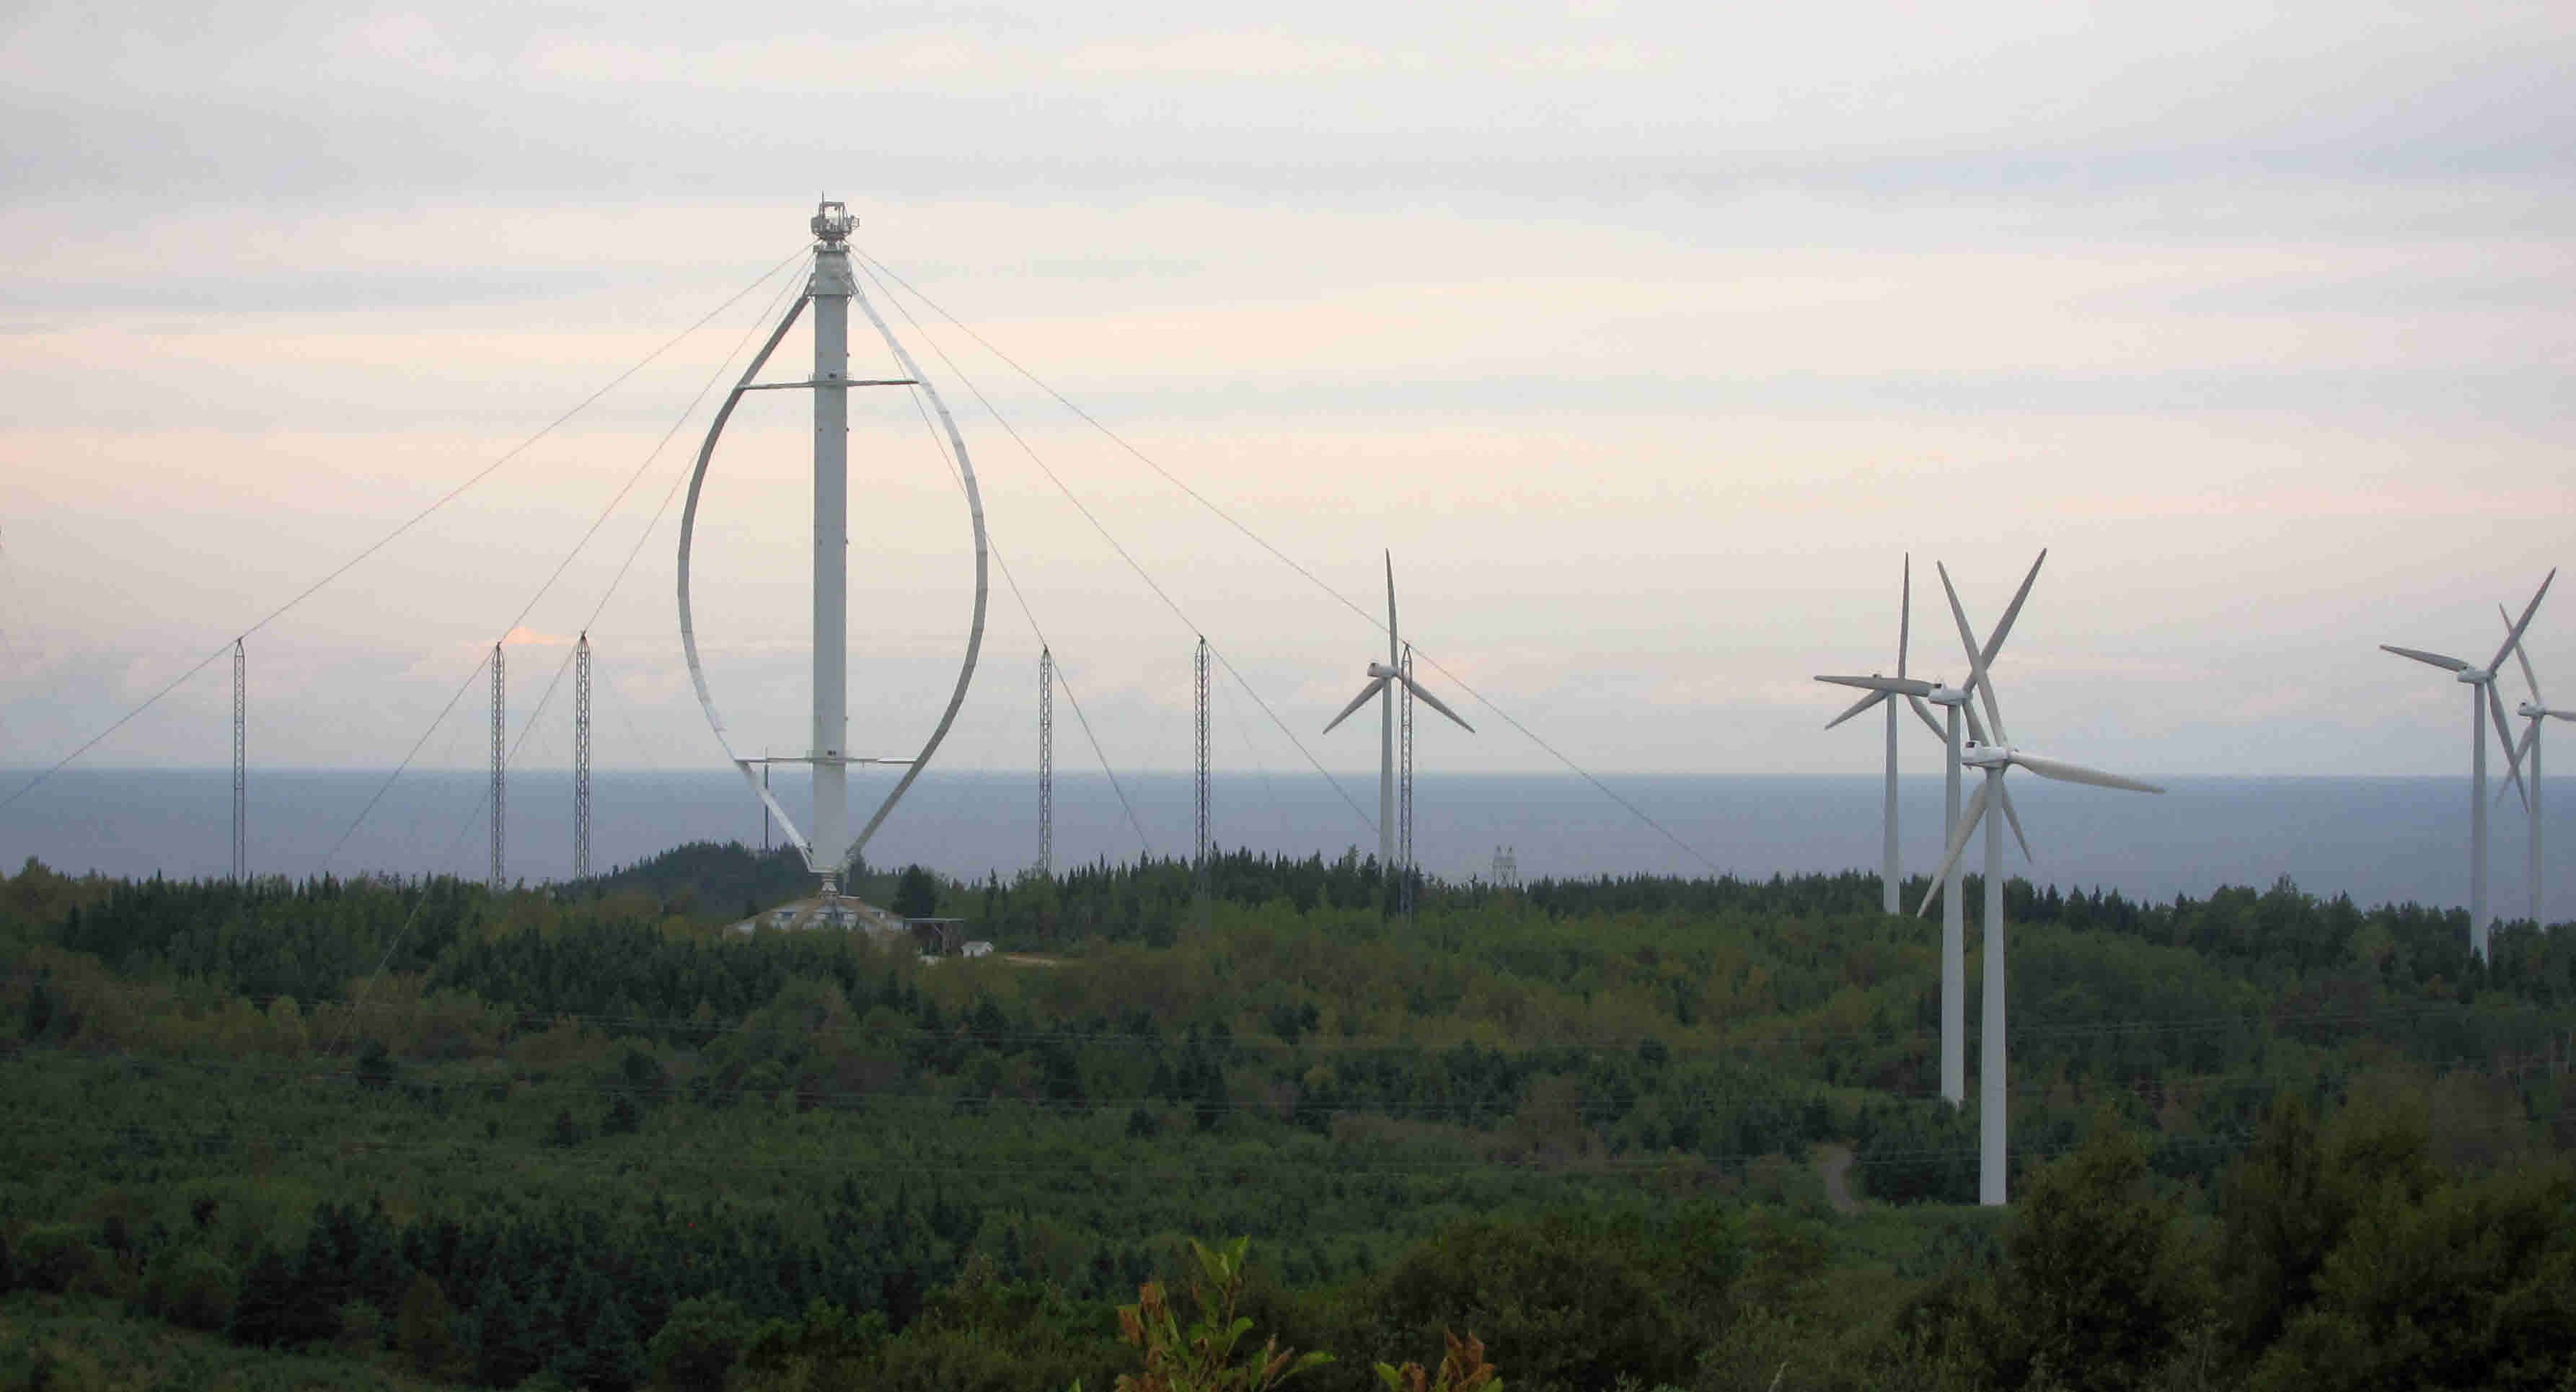
\includegraphics[width=0.9\textwidth]{Imagenes/Eole_cap-chat.jpeg}
    \caption{\small{\textbf{Aerogeneradores de eje vertical y horizontal:} Pierre5018, CC BY-SA 4.0 (https://creativecommons.org/licenses/by-sa/4.0), vía Wikimedia Commons}}
    \label{VAWT}
\end{figure}

Los aerogeneradores de eje horizontal tienen 3 componentes principales: la torre, el rotor y 
la góndola (\emph{nacelle}). Dentro de la góndola se encuentra el generador eléctrico conectado 
con el rotor por medio de los ejes de alta y baja velocidad, así como la caja de cambios 
(\emph{gearbox}) \cite{Pao2009}. La mayoría de las turbinas eólicas de gran escala cuentan con 
un sistema que permite girar la góndola y el rotor para que apunte siempre en la dirección del 
viento, este sistema es manejado por el \emph{yaw actuator} y une la góndola con la torre. El 
rotor incluye las aspas y, en algunos casos, los actuadores que controlan el ángulo de estas 
(\emph{pitch actuator}). 
\\

Las turbinas eólicas pueden ser de velocidad fija o variable. Las turbinas de velocidad variable 
puede trabajar más cerca de la máxima eficiencia aerodinámica por un mayor tiempo. Sin embargo, 
el hecho de tener una velocidad variable implica también que se debe realizar una correcta 
regulación y procesamiento de la electricidad generada para que esta pueda ser subida a la 
red con la frecuencia correcta \cite{Pao2009}.
\\

Las turbinas de velocidad variable suelen trabajar en 3 regiones de operación. Cuando la 
velocidad del viento es baja (usualmente menor a 6 $\text{m}/\text{s}$) la potencia del viento 
es insuficiente y las turbinas suelen permanecer detenidas. A esto se le conoce como \textbf{región 1} 
e incluye también el momento en el que las turbinas se encienden y comienzan a girar. Durante 
la región 1 el control se limita al monitoreo y supervisión de la velocidad del viento para 
determinar en qué momento se pueden iniciar las rutinas de activación para encender las turbinas \cite{Johnson2004}.
\\

La \textbf{región 2} de operación ocurre generalmente cuando el viento alcanza velocidades 
entre 5 y 14 $\text{m}/\text{s}$. En esta región se busca extraer la mayor potencia posible 
del viento y para esto se pueden utilizar cualquiera de los tipos de control disponibles en 
el aerogenerador (\emph{yaw control}, \emph{pitch control} y \emph{torque control}). Debido 
a que las velocidades del viento son menores que las presentadas en la región 3 normalmente 
no es necesario reducir las cargas [mecánicas y eléctricas] cuando la turbina opera en la 
región 2 \cite{Johnson2004}.
\\

Por último, la \textbf{región 3} ocurre cuando el viento supera la velocidad a la cual se 
extrae la potencia máxima por el aerogenerador. Aunque la velocidad del viento siga aumentando, 
las turbinas deben limitar la potencia que se extrae del viento para evitar daños en sus 
componentes debido al estrés y las cargas producidas por la fuerza del viento 
\cite{Pao2009}-\cite{Johnson2004}. De aquí que la gráfica potencia-velocidad se vea plana 
en la región 3 (ver figura \ref{Regiones}) aun cuando el viento se siga incrementando hasta 
alcanzar un cierto valor límite (\emph{high wind cutout}). Después de este límite las turbinas 
deben ser detenidas completamente.
\\
\begin{figure}[H]
    \centering
    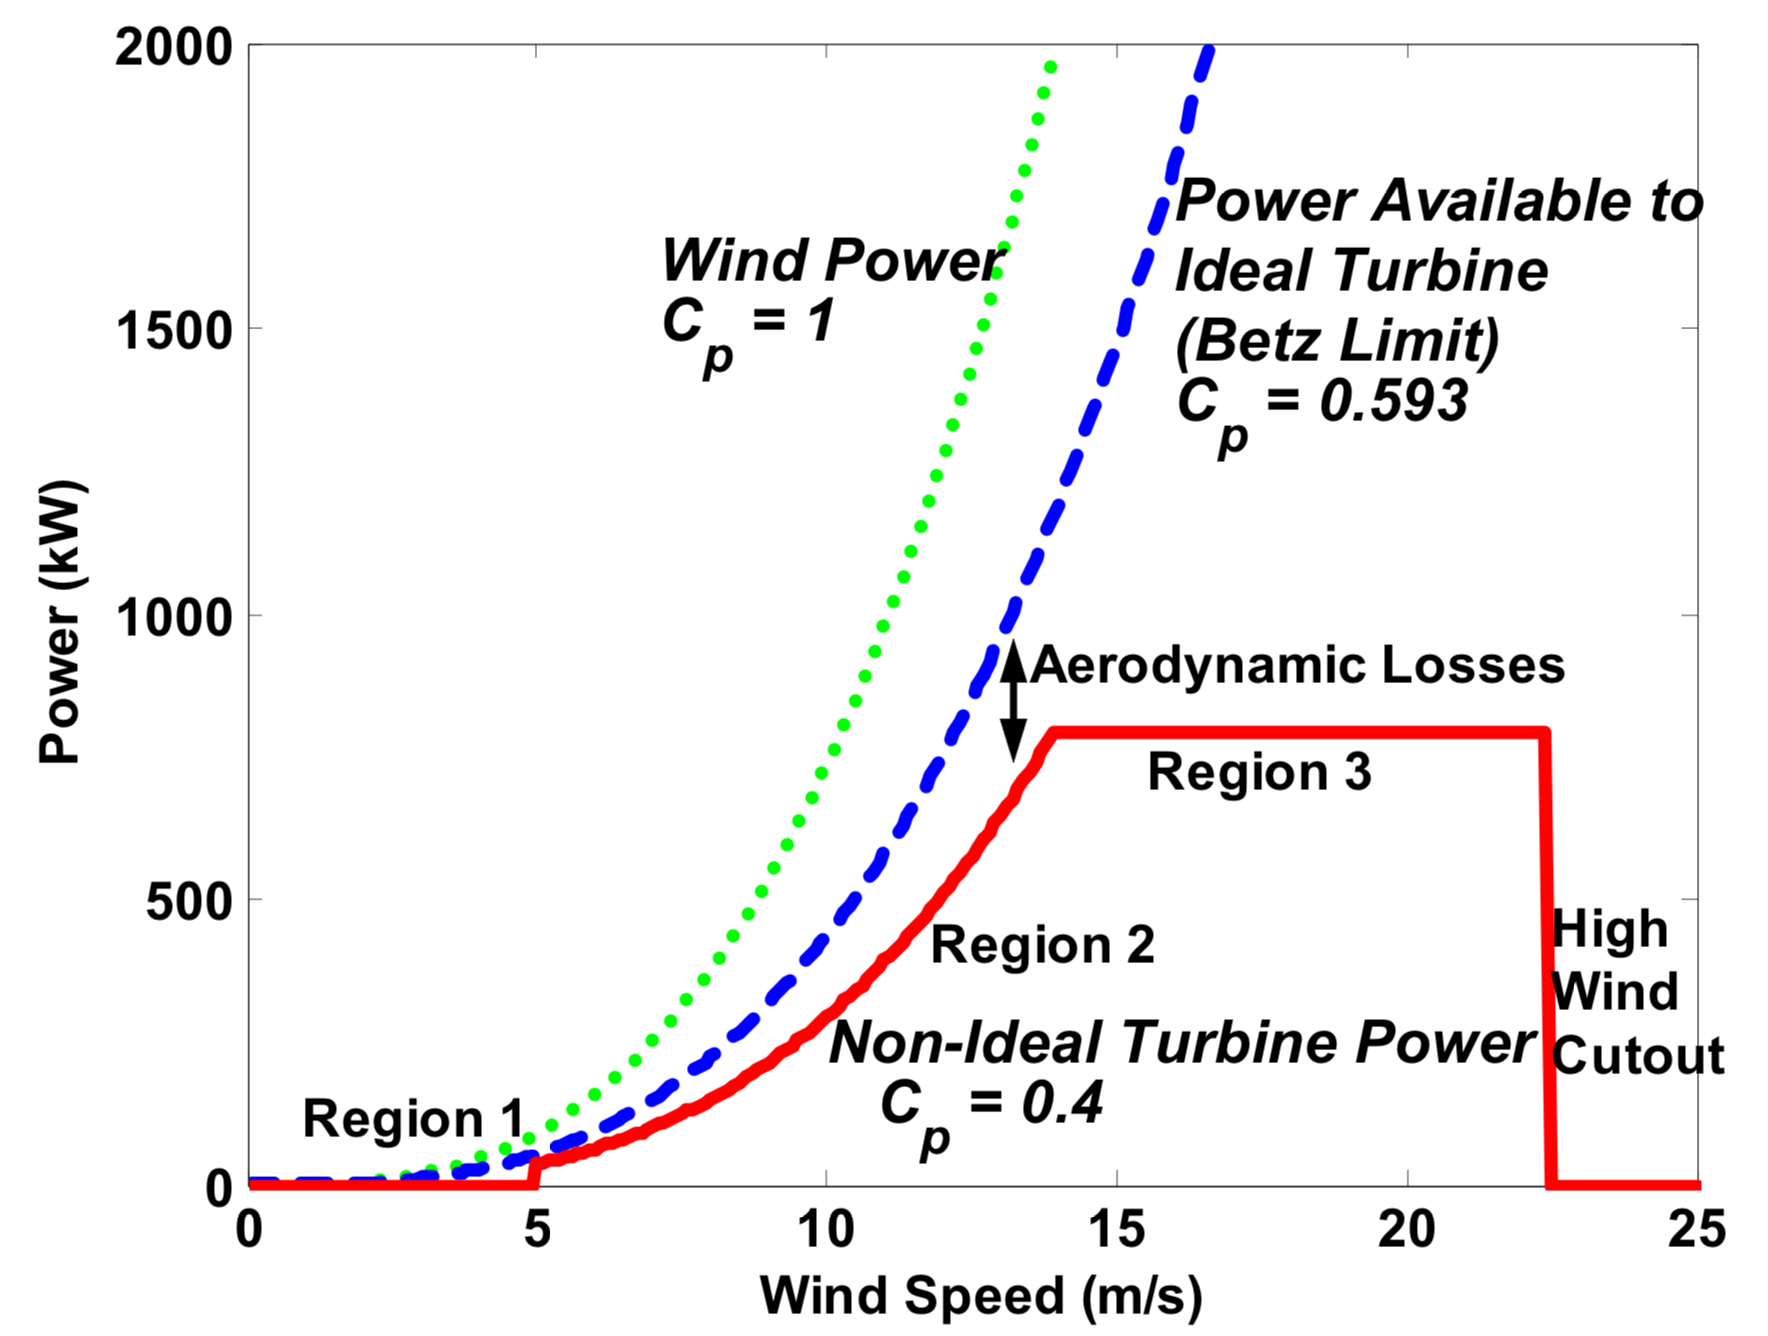
\includegraphics[width=0.8\textwidth]{Imagenes/Regions.jpeg}
    \caption{Regiones de control de un aerogenerador \cite{Johnson2004}}
    \label{Regiones}
\end{figure}

Adicionalmente, las turbinas eólicas tienen una eficiencia definida como el porcentaje de la 
potencia del viento que de hecho puede ser aprovechada por la turbina eólica. La eficiencia 
máxima alcanzable de manera teórica está dada por el número de Betz $B=\frac{16}{27}\approx 
59.26$\% \cite{Huleihil2012}. Esto implica que solo el 59\% de la potencia del viento puede 
ser realmente convertida en energía eléctrica. Este valor es teórico y en la práctica las 
turbinas eólicas suelen tener valores de eficiencia entre 35-45\%.
}

\section{Identificación del problema}
{\parindent0pt
El problema del control de una turbina eólica puede ser tratado desde distintos ángulos. 
Aquella magnitud física que se maneje como variable de control definirá el alcance y el tipo 
del control que se vaya a realizar. 
\\

Las turbinas eólicas producidas en los últimos años incluyen actuadores para cada una de 
las aspas, lo que provee una nueva forma de controlar la generación de energía además de 
la forma tradicional que implica el control del par eléctrico del generador \cite{Laks2009}.
\\

Durante el ciclo de operación de un aerogenerador, este debe poder adaptarse a los cambios 
constantes e impredecibles del viento, tanto en su dirección como en su velocidad. Para esto 
se han implementado sistemas de control que van desde el \emph{yaw control} que permite que 
el conjunto completo de la góndola y el rotor giren sobre la torre para que mantener el 
viento normal al plano del rotor; hasta el \emph{pitch control} que permite girar las aspas 
para modificar el ángulo con el que el viento choca contra la superficie aerodinámica de cada aspa. 
\\

Otra forma de enfrentar el problema de la velocidad del viento —y, por tanto, del torque 
recibido por el rotor— es a través de controlar el par eléctrico del generador (\emph{torque control}), 
lo que permite controlar la cantidad de torque que se demanda del rotor y de esta forma 
optimizar su velocidad \cite{Johnson2004}.
\\

Cuando el viento muestra velocidades por debajo del límite establecido para ciertos 
aerogeneradores en específico, estos suelen realizar el control de velocidad del rotor 
por medio del \emph{yaw control} y el control del par eléctrico, manteniendo el ángulo 
de ataque de las aspas a un valor fijo calculado como el óptimo en el cual se extrae la 
mayor cantidad de energía del viento. Sin embargo, cuando el viento alcanza velocidades 
más altas que el valor límite se vuelve importante reducir las cargas mecánicas y 
eléctricas para no superar sus valores máximos considerados en el diseño de dichos componentes. 
\\

La principal consecuencia de alcanzar las velocidades límites del viento es que usualmente 
conlleva a que los aerogeneradores sean frenados hasta quedar completamente detenidos. 
Lo anterior para evitar daños a sus componentes debido a las cargas excesivas, considerando 
además que las turbinas eólicas modernas tienen costos bastante altos asociados tanto a 
su producción como a su mantenimiento. Esto puede resultar contraproducente dado que los 
aerogeneradores permanecen detenidos en aquellos momentos en que la generación de energía 
eléctrica es teóricamente mayor y, por tanto, se está desperdiciando toda esa potencia del viento.


}


\section{Objetivo}
\noindent De lo anterior, la presente tesis tiene como objetivos los siguientes puntos:
\begin{enumerate}
\item Encontrar una ley de control que, manipulando el ángulo de ataque de las aspas, 
permita regular el par mecánico.
\item Considerar el escenario en el que se requiere extraer la máxima potencia proveniente 
del viento, procedimiento conocido como MPTT (Maximum Power Point Tracking). Este punto 
requiere que el aerogenerador rote a cierta velocidad que en la práctica se desconoce.
\item Agregar al modelo la parte eléctrica y encontrar una ley de control que permita 
regular el par eléctrico al manipular la carga. Luego, hacer operar de manera conjunta 
ambas partes, la eléctrica y la mecánica, con sus respectivas leyes de control. 
\end{enumerate}


\section{Metodología}

\noindent Para el desarrollo de esta tesis se seguirán la metodología ágil. En particular 
la variante de la metodología ágil conocida como SCRUM. La elección debido a que su 
organización en \emph{sprints} cortos con versiones listas para entregar permite 
enfocar la atención en un problema a la vez y trabajar sobre este hasta resolverlo. 
De esta forma el esfuerzo se concentra en una etapa del proyecto y hasta que esta 
esté concluida se avanza con las posteriores. La metodología ágil SCRUM facilita 
también el desarrollo de proyectos de alta complejidad y en los que se incursiona 
en áreas poco conocidas para los colaboradores. 
%!TEX root = ../main.tex
\chapter{Análisis}

En este capítulo se introduce formalmente el problema de control del \emph{pitch angle} en las turbinas eólicas. Se detallan las aproximaciones que ha habido para los distintos tipos de control que se pueden realizar en una turbina eólica (principalmente \emph{pitch control} y \emph{torque control}) a través de los años y los resultados que han tenido (\emph{state of the art}). Además, se enuncian los requerimientos y las restricciones para el diseño del controlador. Por último, se mencionan los estándares que existen tanto a nivel nacional como internacional que estén relacionados o que puedan afectar el diseño del controlador.

\section{Requerimientos}
{\parindent0pt
El controlador debe responder adecuadamente ante los cambios en las condiciones del viento. Se debe monitorear (sensar) la velocidad para determinar en qué momento se pasa de una región de operación a otra. El \emph{pitch control} debe responder a la señal del control supervisor cuando la turbina entre en la región 3 de operación y su función es la de disminuir (o aumentar) la potencia recibida del viento. Para esto, cuando el control supervisor determine que la carga mecánica en el rotor es cercana a un valor límite (con una tolerancia para fines de seguridad) el \emph{pitch control} debe abatir las aspas, reduciendo así el ángulo de ataque de estas, y permitiendo que el viento pase por el área de barrido del rotor generando un menor empuje en las aspas. Por el contrario, cuando la velocidad del rotor haya disminuido por debajo de un cierto umbral, las aspas deben girar nuevamente a la posición de máxima extracción de potencia. 
\\

La tarea de control es permitir que el aerogenerador siga operando por un mayor tiempo durante condiciones climáticas con vientos de alta velocidad antes de tener que ser frenado totalmente para evitar daños. Esto tiene como objetivo aprovechar de manera más eficiente los escenarios con vientos más rápidos para extraer en estos momentos mayor energía que durante la operación del aerogenerador en condiciones normales. Dichas condiciones de viento “extremo” suelen ocurrir con baja frecuencia a lo largo de un cierto periodo de tiempo (por lo general un año), y dependen principalmente de la ubicación geográfica del parque eólico donde esté instalada la turbina. Parte fundamental del desarrollo de este trabajo implica el diseño de un controlador que sea factible de implementar en cualquier ubicación geográfica, pero particularmente en aquellas donde se presentan vientos de alta velocidad con mayor frecuencia a lo largo del año.
\\

Se requiere, de igual forma, evaluar la conveniencia de la implementación del sistema de control en términos de su gasto energético en comparación con el incremento en la producción debido a su uso. Esto pensando en que el hecho de agregar un grado de libertad a partir de controlar el \emph{pitch angle} debería provocar un incremento en la generación de energía eléctrica mayor a su consumo debido al uso de los actuadores —consumo que debe ser bajo debido a la naturaleza hidráulica del mecanismo—. Sí lo anterior no se cumple, lo cual puede deberse a la baja frecuencia de vientos de alta velocidad o a la ineficiencia del controlador para aprovechar dichos vientos, entonces se concluiría que el grado extra de libertad debido al control del ángulo de las aspas no es adecuado para un aerogenerador con sus condiciones particulares. 

}

\section{Restricciones}
{\parindent0pt
Dado que el objetivo de la tesis es el diseño de un controlador (a partir de encontrar la ley de control) para el ángulo de ataque de las aspas de la turbina (\emph{pitch angle}) y debido a lo complicado —o incluso inviable— de ser implementado en un aerogenerador real, el resultado esperado para esta tesis será la simulación de la operación de la turbina bajo diferentes condiciones que permita observar el trabajo de los sistemas de control durante las 3 regiones de operación de la turbina. Para esto la simulación debe permitir variar las condiciones del viento simuladas (velocidad y dirección) a lo largo de un periodo determinado de tiempo y, como resultado, se debe observar el comportamiento esperado de la turbina de acuerdo a la región en la que se encuentre operando. 
\\

Es de particular interés la región 3 de operación debido a que es donde el viento tiene velocidades más altas e interesa observar el trabajo del controlador para evaluar su eficiencia al momento de reducir la carga mecánica que recibe el rotor debido al viento. Dado que uno de los objetivos de la tesis es extender el tiempo de operación de la turbina en la región 3 (para incrementar la cantidad de energía eléctrica producida) es indispensable que la simulación muestre de manera precisa el rango de tiempo desde que se entra en la región 3 hasta que ocurre el corte por exceso de velocidad (\emph{high speed cut}).
\\

La simulación se hará en Matlab Simulink y deberá presentar tanto una representación visual de la operación de las turbinas como los datos asociados a dicha operación ya sea en tablas o gráficas, según sea conveniente en cada caso. Para las características de la turbina se seguirán seguirá una línea de diseño de algún aerogenerador ya existente. Obteniendo a partir de este diseño algunos datos relevantes como la medida de las aspas (para el área de barrido del rotor). Así mismo, debido a que las condiciones del viento son diferentes en cada región geográfica, se busca que el comportamiento del viento en la simulación pueda emular con cierto grado de certeza las condiciones de algún lugar real en donde se realice la operación de turbinas eólicas. Un ejemplo de lo anterior es el tramo La Venta-La Ventosa en la región del Istmo de Tehuantepec en el estado de Oaxaca.
\\

Lo anterior con es principalmente con fines de visualización y de ejemplificación, dado que el diseño del controlador pretende ser general y no estar enfocado a un tipo específico de turbinas o diseñado para trabajar en alguna región con ciertas características climáticas en particular. 

}
\section{Trabajos relacionados}
{\parindent0pt 
El diseño de controladores para turbinas eólicas de velocidad variable se suele realizar desde dos puntos de partida: controladores con un enfoque más teórico que suelen resultar en un control más avanzado y preciso pero que funciona sobre una turbina en la que se han simplificado muchas cosas; y un enfoque más práctico que suele resultar en una turbina mejor modelada y, por lo mismo, con menor precisión al momento de operar \cite{Johnson2004}. Ambas situaciones suelen deberse al hecho de que la mayoría de las investigaciones que derivan en el diseño de controladores de velocidad concluyen en la construcción de simulaciones en las que las leyes de control expuestas funcionan bien, mas no es común que dichos controladores sean probados en turbinas reales.
\\

Para el \emph{pitch control} ha habido desde aproximaciones clásicas como lo es el uso de controladores PID \cite{Johnson2004}. Investigaciones más recientes han apuntado también al uso de controles adaptativos para el control de velocidad del rotor, aunque no han sido suficientemente probados en campo \cite{Johnson2004}. Algunas otras investigaciones han buscado alternativas a los \emph{pitch actuators} para cambiar la aerodinámica de las aspas, explorando el uso de \emph{micro-tabs} y pequeñas válvulas de aire presurizado que permite un flujo extra de aire en la superficie de las aspas y, de esta forma, cambiar el flujo de aire que cruza el área de barrido del rotor \cite{Pao2009}.
\\

Una aproximación más actual se hace en \cite{Jie2020} a partir del uso de redes neuronales y modelos predictivos tomando como entradas varios parámetros de medidos por las turbinas. A partir de esto, se utilizan modelos de aprendizaje como ELM (Extreme Learning Machine). Las salidas son tratadas como datos de referencia para el \emph{pitch control}.
\\

Se ha explorado también el uso de nuevas tecnologías que permitirían nuevas posibilidades en el diseño de controladores. Un ejemplo de esto es el uso de sensores LIDAR (del inglés \emph{Light Detection and Ranging}) para fines de medición del viento. Los sensores \emph{lidar} han sido usados exitosamente con aplicaciones meteorológicas y podrían ser interesantes de aprovechar en el control de granjas eólicas. Igualmente, turbinas más grandes han empezado a incluir actuadores independientes para cada una de las aspas, lo que permite variar el ángulo de cada una de manera independiente. Esto posibilita toda una nueva forma de realizar el control de velocidad del rotor \cite{Pao2009}. 

}


\section{Estándares de la industria}
{\parindent0pt 
El diseño de estándares para la fabricación de turbinas eólicas comienza en 1986 cuando Germanischer Lloyd publicó un conjunto de regulaciones para la certificación del diseño de turbinas eólicas que, conforme las investigaciones alrededor de este campo fueron aumentando, llevaron a la publicación en 1993 de la \emph{Regulation for the Certification of Wind Energy Conversion Systems}. Similarmente se publicaron estándares de carácter nacional en Países Bajos (NEN 6096) en 1988 y en Dinamarca (DS 472) en 1992 \cite{Burton2011}.
\\

La primera emisión de normas con un carácter verdaderamente internacional fue llevada a cabo por la \emph{International Electrothecnical Comission (IEC)} en 1988 y culminó con la publicación de las normas \emph{IEC-1400-1 Wind Turbine Generator Systems – Part 1: Safety Requirements}. Posteriores revisiones y ediciones fueron publicadas. Entre ellas la IEC-61400 publicada en 2005 y que continua actualmente en funcionamiento luego de varias revisiones \cite{Burton2011}.
}

\section{Plan de trabajo}

\textbf{Fechas de entregas:}
\begin{itemize}
    \item \emph{Capítulos I y II:} 29 de noviembre, 2023.

    \item \emph{Capitulo III:} 28 de febrero, 2024.

    \item \emph{Capítulo IV:} 01 de abril, 2024.

    \item \emph{Capítulos V y VI:} 15 de mayo, 2024. 
\end{itemize}

\include{Capitulos/Diseño}
%\include{Capitulos/Implementación}
%\chapter{Pruebas y resultados}

En este capítulo se describen los resultados obtenidos en cada parte de la implementación de la solución así como las pruebas realizadas y los resultados de éstas con el fin de proporcionar la información adecuada para saber si se cumplieron los requerimientos de esta tesina. 
\section{Pruebas realizadas y sus resultados}
Lorem ipsum dolor sit amet, consectetur adipiscing elit, sed do eiusmod tempor incididunt ut labore et dolore magna aliqua. Ut enim ad minim veniam, quis nostrud exercitation ullamco laboris nisi ut aliquip ex ea commodo consequat.
Lorem ipsum dolor sit amet, consectetur adipiscing elit, sed do eiusmod tempor incididunt ut labore et dolore magna aliqua. Ut enim ad minim veniam, quis nostrud exercitation ullamco laboris nisi ut aliquip ex ea commodo consequat.
Lorem ipsum dolor sit amet, consectetur adipiscing elit, sed do eiusmod tempor incididunt ut labore et dolore magna aliqua. Ut enim ad minim veniam, quis nostrud exercitation ullamco laboris nisi ut aliquip ex ea commodo consequat.Lorem ipsum dolor sit amet, consectetur adipiscing elit, sed do eiusmod tempor incididunt ut labore et dolore magna aliqua. Ut enim ad minim veniam, quis nostrud exercitation ullamco laboris nisi ut aliquip ex ea commodo consequat.
%\chapter{Conclusiones} \label{intro_chapter}

En este capítulo se analizan los resultados de las pruebas realizadas para determinar si la solución proporcionada de esta tesis cumple con los requerimientos de la misma. 

\section{Conclusiones pruebas de velocidad y posición}
Lorem ipsum dolor sit amet, consectetur adipiscing elit, sed do eiusmod tempor incididunt ut labore et dolore magna aliqua. Ut enim ad minim veniam, quis nostrud exercitation ullamco laboris nisi ut aliquip ex ea commodo consequat.Lorem ipsum dolor sit amet, consectetur adipiscing elit, sed do eiusmod tempor incididunt ut labore et dolore magna aliqua. Ut enim ad minim veniam, quis nostrud exercitation ullamco laboris nisi ut aliquip ex ea commodo consequat.Lorem ipsum dolor sit amet, consectetur adipiscing elit, sed do eiusmod tempor incididunt ut labore et dolore magna aliqua. Ut enim ad minim veniam, quis nostrud exercitation ullamco laboris nisi ut aliquip ex ea commodo consequat.Lorem ipsum dolor sit amet, consectetur adipiscing elit, sed do eiusmod tempor incididunt ut labore et dolore magna aliqua. Ut enim ad minim veniam, quis nostrud exercitation ullamco laboris nisi ut aliquip ex ea commodo consequat.Lorem ipsum dolor sit amet, consectetur adipiscing elit, sed do eiusmod tempor incididunt ut labore et dolore magna aliqua. Ut enim ad minim veniam, quis nostrud exercitation ullamco laboris nisi ut aliquip ex ea commodo consequat.Lorem ipsum dolor sit amet, consectetur adipiscing elit, sed do eiusmod tempor incididunt ut labore et dolore magna aliqua. Ut enim ad minim veniam, quis nostrud exercitation ullamco laboris nisi ut aliquip ex ea commodo consequat.

%----------------------------------------------------------------------------------------
%	Apéndices
%----------------------------------------------------------------------------------------

\appendix
%\chapter{Apéndices}


%----------------------------------------------------------------------------------------
%	Bibliografía
%----------------------------------------------------------------------------------------
%\printbibliography[notcategory=cited, title={Referencias}]
%\printbibliography[title = {Referencias}]
\renewcommand\bibname{Referencias}
\bibliography{Referencias/Documentos/references}
\bibliographystyle{ieeetr}

\end{document}